\documentclass[10pt]{beamer}
% Class options include: notes, notesonly, handout, trans,
%                        hidesubsections, shadesubsections,
%                        inrow, blue, red, grey, brown

% Theme for beamer presentation.
\usepackage{beamerthemesplit} 
%\usepackage{times}
\usepackage{anysize}
\usepackage{fancyhdr}
\usepackage{graphicx}
\usepackage{pdfpages}
\usepackage[fleqn]{amsmath}
\usepackage{amssymb}
% Other themes include: beamerthemebars, beamerthemelined, 
%                       beamerthemetree, beamerthemetreebars  

\title{Jafar --- Intelligent Othello Agent}    % Enter your title between curly braces
\author{Joshua Nelson, Tim Cosgrove, Andrew Haigh}                 % Enter your name between curly braces
\institute{COMP3130 Research Project}      % Enter your institute name between curly braces
\date{\today}                    % Enter the date or \today between curly braces

\usetheme{PaloAlto}
\usecolortheme{crane}

\newcommand{\bcen}{\begin{center}}
\newcommand{\ecen}{\end{center}}

\begin{document}

% Creates title page of slide show using above information
\begin{frame}
  \titlepage
\end{frame}
\note{} % Add notes to yourself that will be displayed when
        % typeset with the notes or notesonly class options

\section[Outline]{}

% Creates table of contents slide incorporating
% all \section and \subsection commands
\begin{frame}
  
  \begin{columns}[c]
  \column{2in}
  \tableofcontents
  \column{2in}
  \framebox{
\includegraphics[height=4cm]{hipsterjafar}}
  \end{columns}
\end{frame}


\section{Problem Overview}

\begin{frame}
  \frametitle{Problem Overview}   % Insert frame title between curly braces
  \begin{columns}[c]
  \column{2in}  % slides are 3in high by 5in wide
  \begin{itemize}
  \item<1-> The Game --- 10x10 Modified Othello
  \item<2-> The Problem --- Intelligent AI player
  \item<3-> Solution basis
  \end{itemize}
  \column{2in}
  \framebox{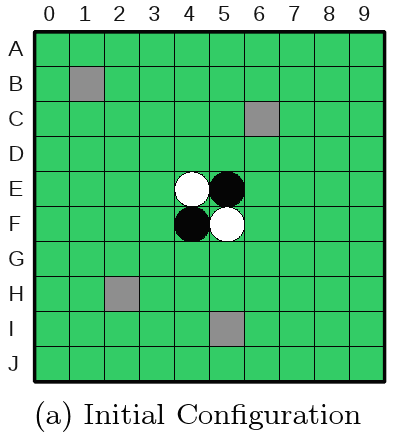
\includegraphics[height=5cm]{initconfig}}
  \end{columns}
\end{frame}

\section{Solution Structure}

\begin{frame}
  \frametitle{Solution Structure}   % Insert frame title between curly braces
  \begin{itemize}
  \item<1-> The MetaPlayer class --- Utilises knowledge of the game state and 
        creates instances of other players accordingly
  \item<2-> NegamaxPlayer (varying depth argument)
  \item<2-> OpeningPlayer
  \item<2-> GreedyPlayer
  \end{itemize}
\end{frame}

\section{Static Evaluation}

\begin{frame}
  \frametitle{Static Evaluation}   % Insert frame title between curly braces
  \begin{itemize}
  \item<1-> The FeatureSet class --- Maintains a list of \emph{features}; functions
  which evaluate a game state based on some criteria of strength
  \item<2-> LegalMoves
  \item<2-> Visibility
  \item<2-> StoneCount
  \item<2-> BlockedAdjacent, CornerPieces, SidePieces
  \end{itemize}
\end{frame}

\section{Learning Algorithms}

\subsection{TD-$\lambda$}

\begin{frame}
  \frametitle{TD-$\lambda$}
  \begin{columns}[c]
  \column{2in}  % slides are 3in high by 5in wide
  \begin{itemize}
  \item<1-> Remaining challenge: decide how important each feature is (the feature 'weights')
  \item<1-> Negative weights not considered (for simplicity)
  \end{itemize}
  \column{2in}
  %\framebox{\includegraphics[height=5cm]{movingAvgChart}}
  \end{columns}
\end{frame}

\subsection{Feature Weight Graphs}

\begin{frame}
  \frametitle{Feature Weight Graphs}
  %\framebox{\includegraphics[height=5cm]{thecharts}}
\end{frame}

\subsection{The EloArena}

\begin{frame}
  \frametitle{The Elo Rankings Arena}
  \begin{itemize}
  \item<1-> Custom made genetic algorithm
  \item<1-> Pits a group of randomly generated agents against each other for Elo style ranking points
  \item<1-> Creates new agents from those who perform best
  \item<2-> Used more as a demonstration of the learning process
  \item<2-> Interesting to see it come to the same conclusions as TD-$\lambda$
  \end{itemize}
\end{frame}

\section{Future Improvements}

\begin{frame}
  \frametitle{Future Improvements}
  \begin{itemize}
  \item<1-> More attention to blocked squares
  \item<2-> Negamax optimisations (better transposition tables, ... etc.)
  \item<3-> Better use of pre-computed data
  \item<4-> More board features (locked squares, open squares, etc.)
  \end{itemize}
\end{frame}

\section{Design Methodology}

\begin{frame}
\frametitle{Design Methodology}
  \bcen
  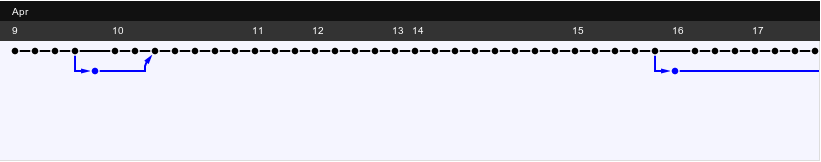
\includegraphics[height=1.3cm,width=7cm]{line1}\\
  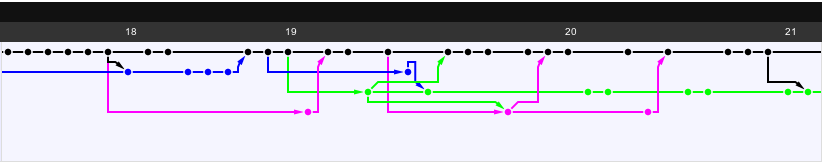
\includegraphics[height=1.3cm,width=7cm]{line2}\\
  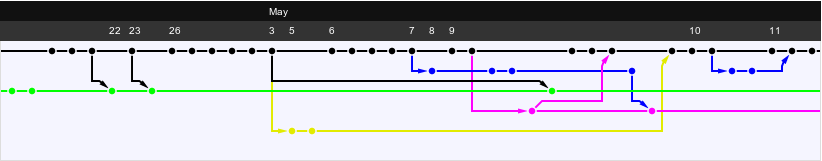
\includegraphics[height=1.3cm,width=7cm]{line3}\\
  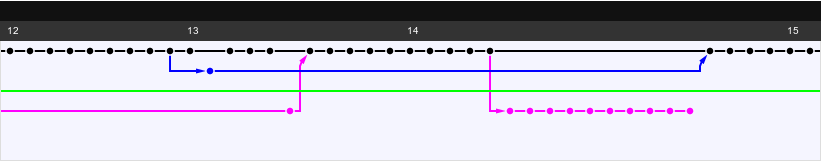
\includegraphics[height=1.3cm,width=7cm]{line4}\\
  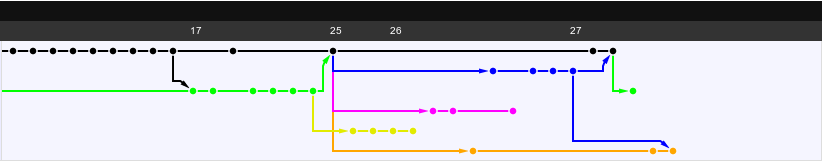
\includegraphics[height=1.3cm,width=7cm]{line5}
  \ecen
\end{frame}


\end{document}
